ICES is in the process of developing methods to identify MSY proxy reference points for data-limited stocks at the ICES Workshop On The Development Of Quantitative Assessment Methodologies Based On Life-History Traits, Exploitation Characteristics, And Other Relevant Parameters For Data-Limited Stocks \href{http://ices.dk/sites/pub/Publication Reports/Expert Group Report/Fisheries Resources Steering Group/2019/WKLIFEIX/WKLIFE_IX_2019.pdf}{(WKLIFE)}. \textbf{MyDas} contributed to this process by proposing and testing new assessment models and methods of establishing reference points and attended both WKLIFE VIII and IX. There are key differences with the ICES approach, however, since \textbf{MyDas} stocks are not currently assessed by ICES and \textbf{MyDas} focused on the available data for each stock first and then on methods, while the ICES approach focuses on the methods first and then applies a limited number of methods to a large number of stocks. 

The importance of the work of \textbf{MyDas} was recognised at WKLIFEVIII where recommendations for \href{http://ices.dk/sites/pub/Publication Reports/Expert Group Report/acom/2018/WKLIFEVIII/WKLIFEVIII_2018.pdf#page=42}{future directions} were made. Following this several examples based on the work of \textbf{MyDas} were made at WKLIFEIX. These included i) the use of life history theory to condition the OM used to evluate the ICES advice rule proposed for \href{http://ices.dk/sites/pub/Publication Reports/Expert Group Report/Fisheries Resources Steering Group/2019/WKLIFEIX/WKLIFE_IX_2019.pdf#page=30}{category 3 and 4 stocks}; ii) Receiver Operating Characteristic (ROC) curves to explore the setting of appropriate 
\href{http://ices.dk/sites/pub/Publication Reports/Expert Group Report/Fisheries Resources Steering Group/2019/WKLIFEIX/WKLIFE_IX_2019.pdf#page=58}{reference levels} in the the catch rule; and iii) the use of trends in an index \href{http://ices.dk/sites/pub/Publication Reports/Expert Group Report/Fisheries Resources Steering Group/2019/WKLIFEIX/WKLIFE_IX_2019.pdf#page=64}{without a reference level}. It was also recommended to use the methods of \textbf{MyDas} to evaluate the robustness of SPiCT based upon the development of Operating Models developed under \href{http://ices.dk/sites/pub/Publication Reports/Expert Group Report/Fisheries Resources Steering Group/2019/WKLIFEIX/WKLIFE_IX_2019.pdf#page=138}{MyDas}.

For stocks with analytical assessments (i.e. category 1 and 2 stocks), the advice rules applied by ICES are consistent with the objective of achieving MSY. For stocks in categories 3 and 4 ICES uses MSY proxy reference points as part of a Precautionary Approach to provide advice on the status of the stock and exploitation. The $F_{MSY}$ proxy corresponds to the exploitation rate that will provide maximum long-term yield, while the $MSY_{Btrigger}$ proxy corresponds to the stock size that triggers a cautious response; i.e. advises a reduced fishing mortality relative to $F_{MSY}$ proxy in order to allow the stock to rebuild. 

%%\\
\textit{Advice Rule}

For stocks with $MSY$ proxy reference points not derived from an assessment model, ICES uses a generic rule of the form 
 
\begin{equation}C_{y+1}=C_{current}rfb\end{equation}

where $C_{current}$ is the catch either in the most recent year available (typically $y-1$) or the average over a number of recent years (e.g. $y-n, ... ,y-1$), $r$ should account for the trend in stock biomass ($r>0$; with $r=1$ if there is no trend), $f$  is a proxy for the ratio $F_{MSY}/$(current explotation) and $b=$ min(1,proxy for the ratio (current stock size)/($MSY_{Btrigger}$)). The later is in effect a hockey stick type HCR. 

$f$ is derived from length based indicators and a number of potential length based reference point and indicators\footnote{\url{'http://ices.dk/sites/pub/Publication Reports/Guidelines and Policies/16.04.03.02_Category_3-4_Reference_Points.pdf'}} have been identified by ICES for stocks in categories 3 and 4 (see Table \ref{tab:lib}) 

\begin{table}[h!]\centering
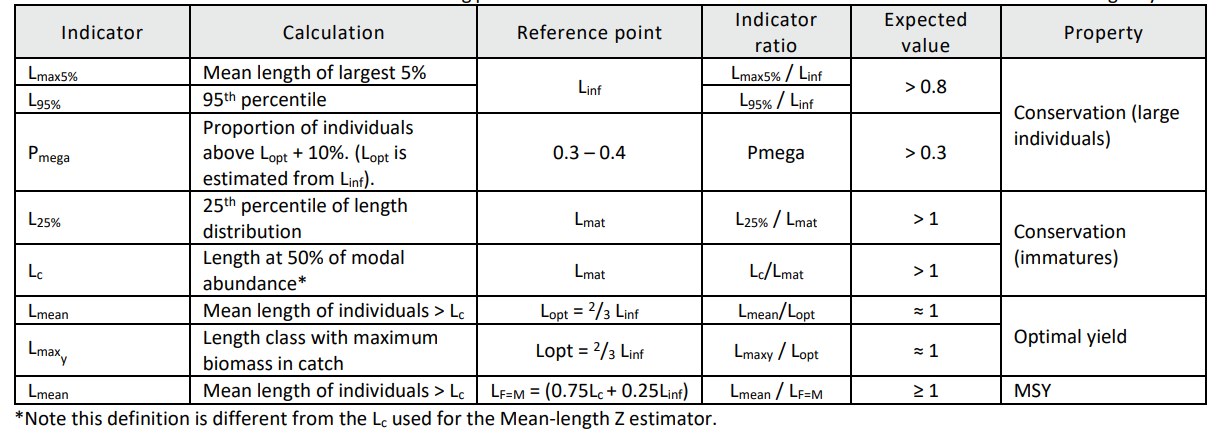
\includegraphics[width=\textwidth]{figs/lib.png}
\caption{Length based indicators.}
\label{tab:lib}
\end{table}

The \textbf{mydas} package includes methods to simulate length frequency data and estimate indicators; Figure \ref{fig:ompollack} shows an OM based on pollack that was used to simulate indicators (Figure \ref{fig:libsim}).

\begin{figure}[h]\centering
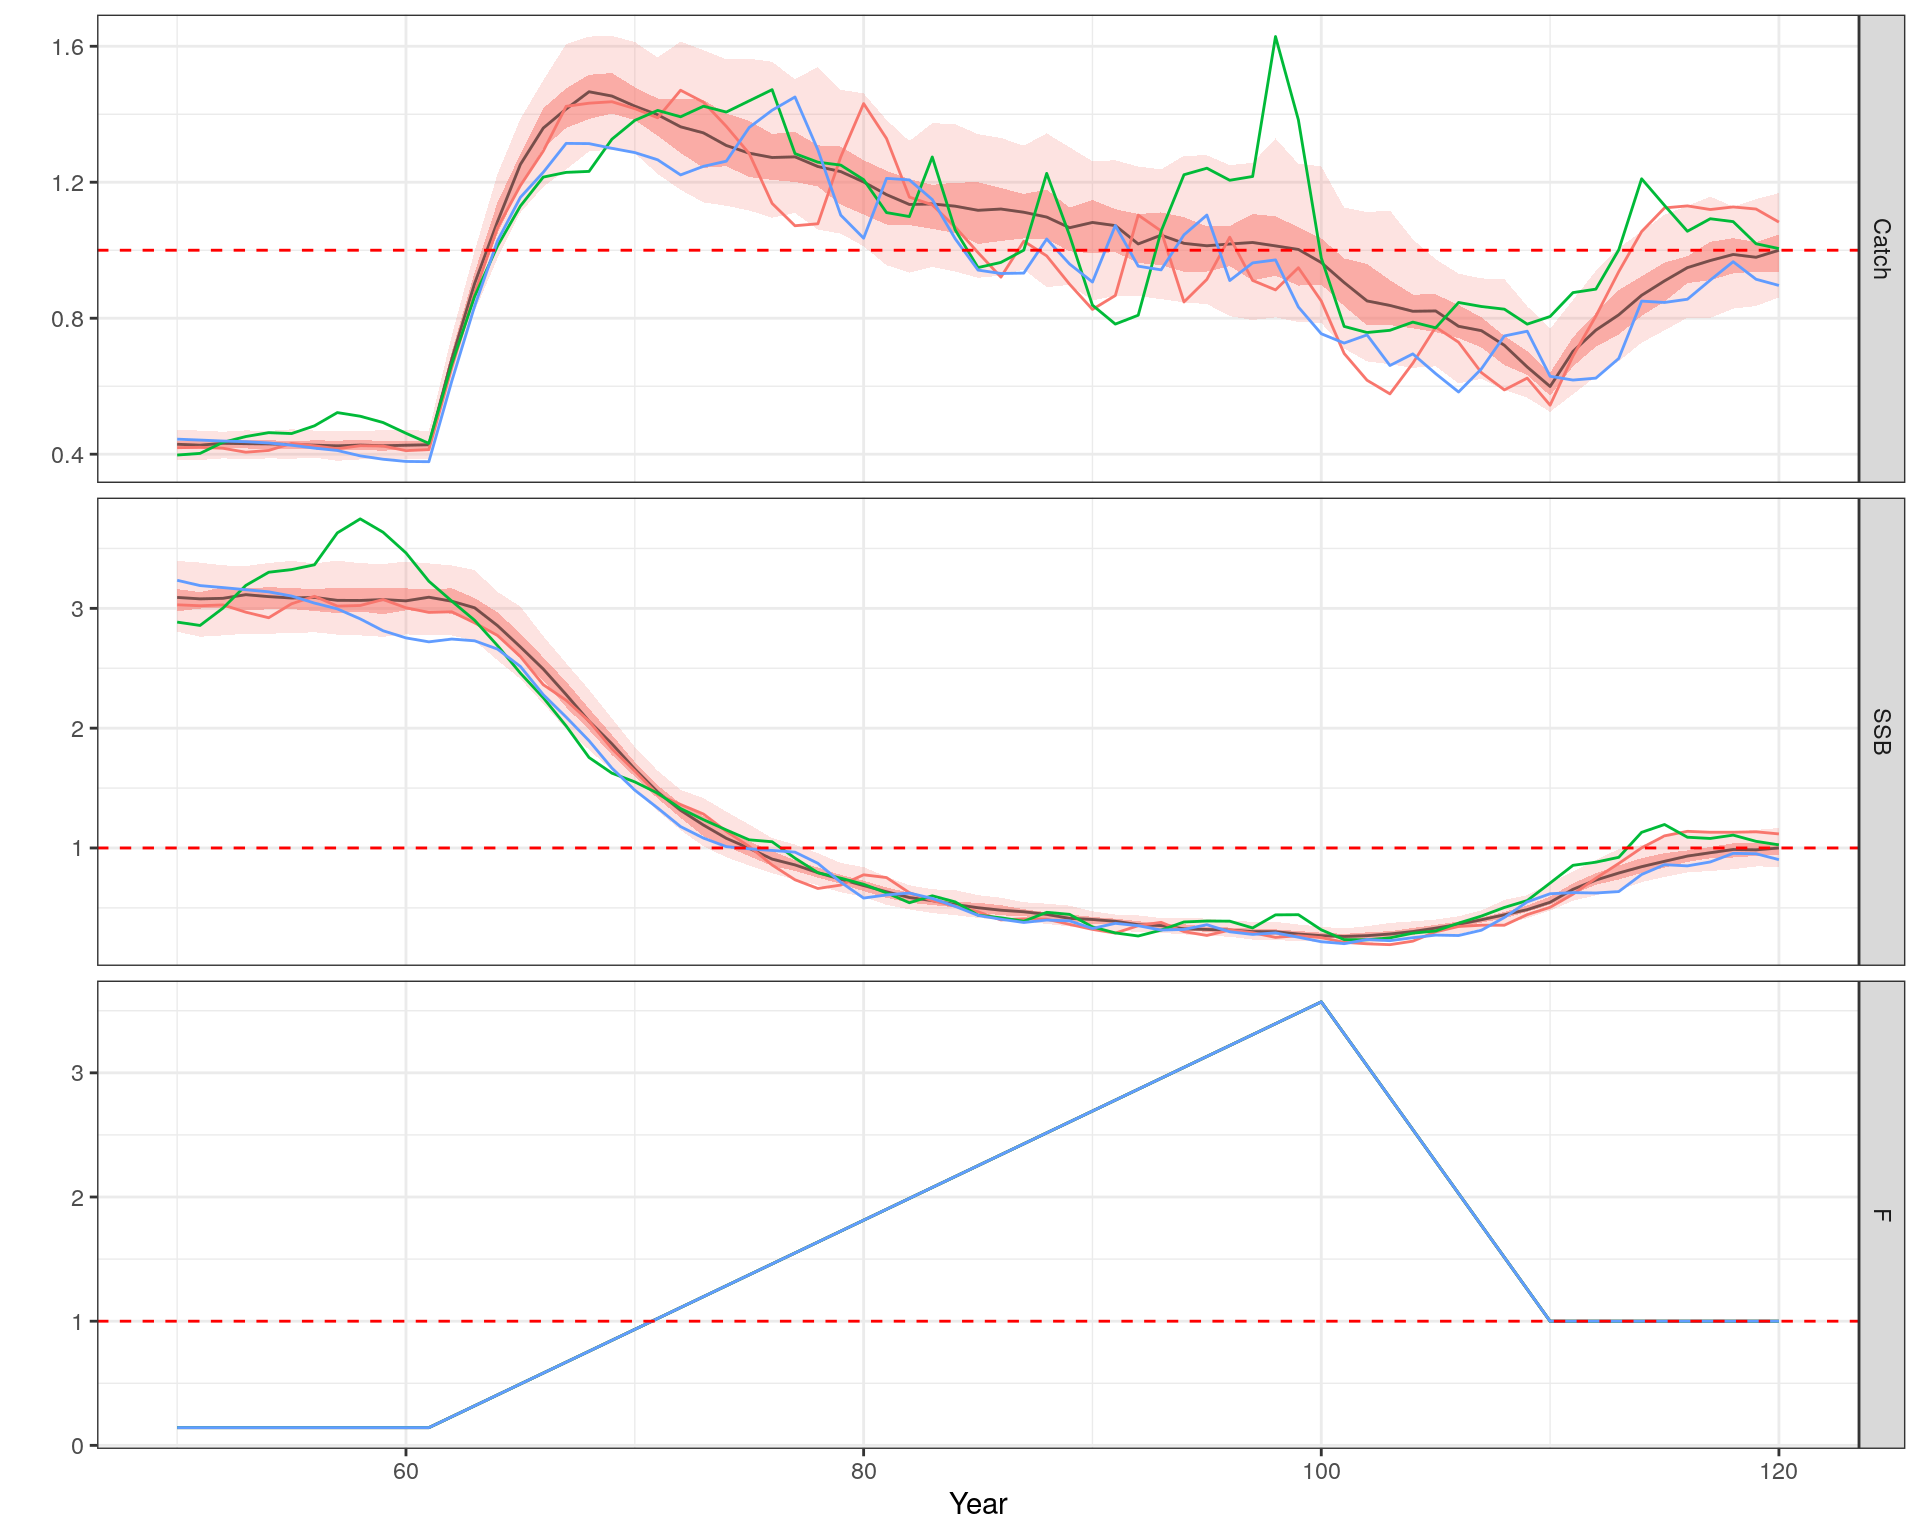
\includegraphics[width=\textwidth]{figs/roc-finalts-pollack-1.png}
\caption{Time series of simulated length based indicators, compared to $F/F_{MSY}$}
\label{fig:ompollack}
\end{figure}

\begin{figure}[h]\centering
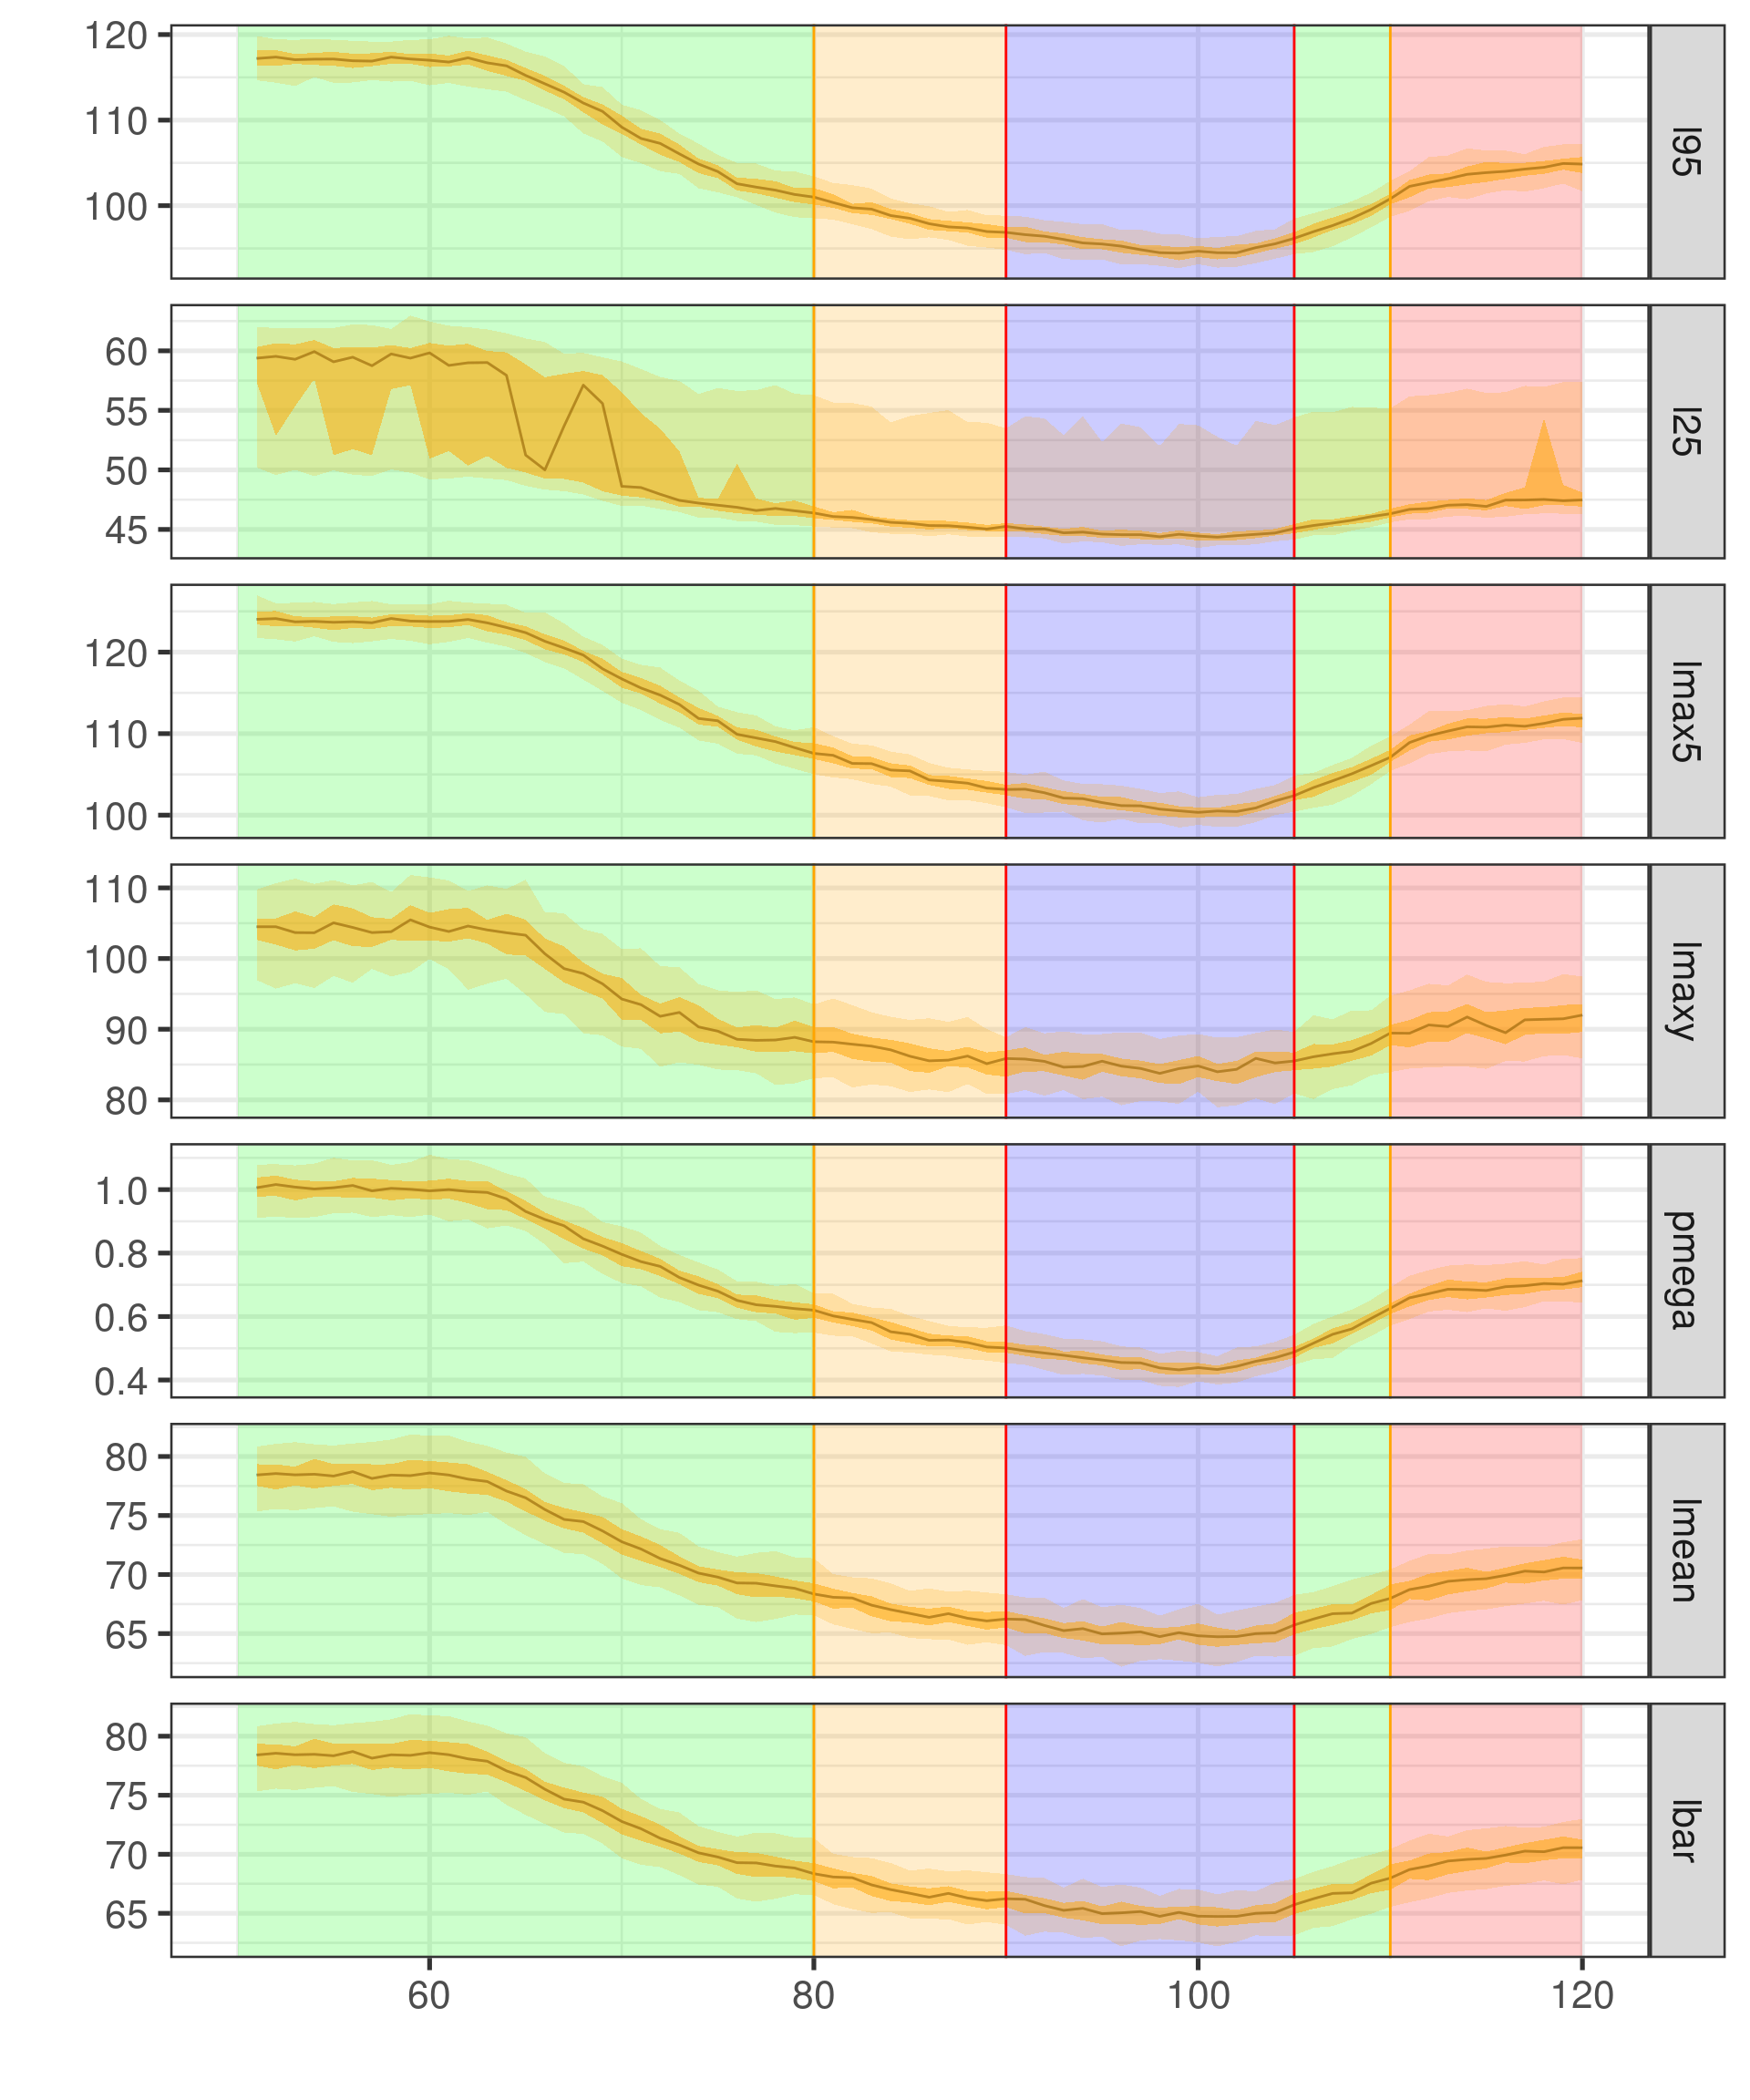
\includegraphics[width=\textwidth]{figs/roc-finalinds-1.png}
\caption{Time series of simulated length based indicators, compared to $F/F_{MSY}$}
\label{fig:libsim}
\end{figure}

To ensure that advice based on such indicators is precautionary, Management Strategy Evaluation was used to evaluate an empirical rule of the form $C_{y+1}=C_{current}rfb$ that bases catch advice on recent catches, information from a biomass survey index ($r$), length based indicators ($f$) and proxy MSY reference point ($b$) \citep{fischer2019hcr}. The OM was conditioned on life histories using the method developed by \textbf{MyDas} .The performance of the rule varied substantially between stocks, and the risk of breaching limit reference points was inversely correlated to the von Bertalanffy growth parameter $k$. Stocks with $k$ >0.32 had a high probability of stock collapse. It was shown that a single generic catch rule cannot be applied across all life-histories, and management should instead be linked to life-history traits, and in particular, the nature of the time series. This supported the premise of \textbf{MyDas} that to develop robust management it is important to consider the nature of the stock dynamics, knowledge and data. 
Counter-intuitively the catch rule performed poorly for the more productive stocks (those with higher $k$) compared to the less productive stocks (with lower $k$). The performance of the catch rule, however, is an emergent property of the interaction between the operating model and the catch rule. Therefore this is an important results which would not have been apparent without the work of our manuscript.

The advised catch was mainly influenced by one component of the rule (the trend in the relative index of abundance) and biomass trends for stocks with higher  are inherently more variable, which in turn leads to higher fluctuations in catch. Therefore when managed by the ICES catch rule, the stocks with higher  were more likely to collapse during simulation. This behaviour can be attributed to an initial rapid recovery, which resulted in an increase in catch. Once the stocks started to decline again, however, catch was not reduced quickly enough to avoid stock collapse. This undesirable feature is caused by the design of the catch rule, which bases the newly advised catch on the previous catch and observed data with a time-lag. Since the less productive stocks (those with low ) were also less variable, the catch rule was sufficiently reactive to avoid stock collapse.

Therefore two papers are currently being drafted. The first used Receiver Operating Characteristic (ROC) curves used to explore the setting of appropriate reference levels in the f component of the catch rule for the \textbf{MyDas} case studies. In particular to explore how these depend on life-history traits and the nature of the time-series. The second evaluated the use of trends in an index without a reference level for pollack. To do this, a Management Strategy Evaluation (MSE) was conducted to evaluate an empirical harvest control rule (HCR) based on a trend in an index of
abundance. The Operating Model (OM) was conditioning on pollack life-history characteristics and the HCR was based on that used by the Commission for the Conservation of Southern Bluefin Tuna (CCSBT). The HCR has several parameters that require tuning \citep{hillary2015scientific}, i.e. the parameters are found by choosing values that best meet the objectives of asset and stakeholders; i.e. optimises the outcomes modelled as a reward function.

